	
\chapter{Introduction}
\label{chap-INTRO}

%%%%%%%%%%%%%%%%%%%%%%%%%%%%%%%%%%%%%%%%%%%%%%%%%%%%%%%%%%%%%%%%%%%%%%%%%%%%%%%%%%%%%%%%%%%%%%%%%%%%%%%%%%%%%%%%%%%%%%%%%%%%%%%%%%%%%%%%%%%%%%%%%%%%%%%%%%%%%%%%%%%%%%%%%%%%%%%
\section{Anderson Model of Localisation}
\label{sec-AML}

  The interest in this thesis is how electrons behave when the disorder in a lattice is sufficiently strong such that it can cause a transition from a metallic to an insulating state.  By disorder, we mean the presence of impurities and distortions, both being randomly distributed in an otherwise perfect (clean and periodic) lattice.  The picture of disorder for a travelling electron is a sea of random potential.  Localisation of electrons happens as an interference effect due to multiple scatterings of the single particle electronic wavefunction with itself by a random potential.  This phenomenon is first demonstrated by Anderson \cite{And58} in his seminal paper on the absence of diffusion in a simple system of noninteracting particles with random site potential energy and zero external fields.
Since then, the Anderson localisation \cite{KraM93,EveM08} is experimentally observed in microwaves \cite{DalASPM91}, ultrasound \cite{HuSPS08,FaeSPLT09}, light waves \cite{WieBLR97,MooPYB08} quantum waves \cite{HasSMI08,RicRMZ10} and cold atoms \cite{RoaDFF08,BilJZB08}.
%
\begin{figure}
  \centering
  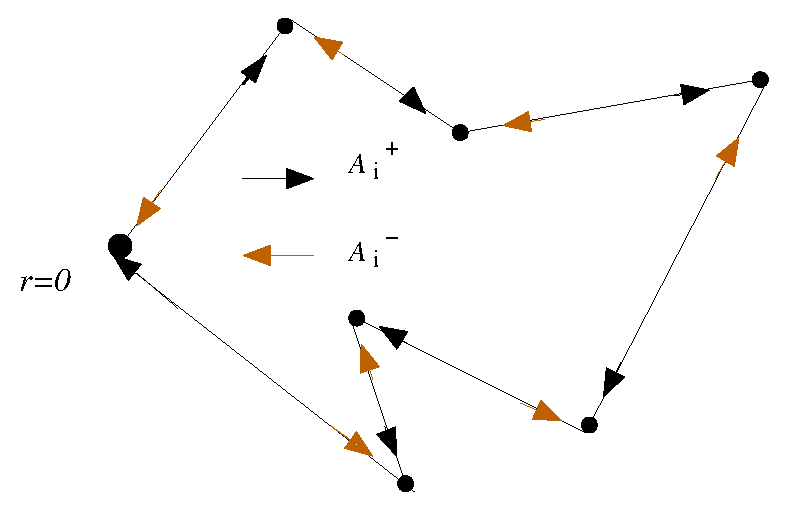
\includegraphics[width=4.5in]{localisation.eps}
   \caption[ A schematic picture of coherent back-scattering of an electron by a random potential.]{  A schematic picture of coherent back-scattering of an electron by a random potential.  An electron returns to its initial position at $r=0$  with probability amplitude $A_i^+(t')$ after a series of scattering events as traced by the black arrows.  The brown arrows trace the corresponding inverse path with probability amplitude $A_i^-(t')$.}
\label{fig-localisation}
\end{figure}
%

If the phase coherence length $l_\varphi$ of the electron is large compared with the system size $L$ then the quantum interference effects become relevant that Anderson localisation for electrons can happen.  This regime is reached when temperature is very low such that inelastic electron-electron and electron-phonon scatterings are suppressed.
%
We can visualize the coherent backscattering that causes localisation in the following manner \cite{Ber83, Ber84}.  We consider an electron at point $\vec{r}=0$ and time $t=0$.  The probability to return to the original point after some time $t=t'$ is given by
%
\begin{equation}
\label{eq-returnPROB}
 \mathcal{P}(t') = \left|\sum_{i\in S}A_i(t')\right|^2,
\end{equation}
%
where $A_i(t')$ is the probability amplitude of an electron that took the $i$th path to return to $\vec{r}=0$ after a number of random scattering events.  The return probability $\mathcal{P}(t')$ is the sum of all possible scattering paths $S$.  Let us consider a simple illustration in Fig.~\ref{fig-localisation}.  For every clockwise path $S_i^+$ traversed by an electron with probability amplitude $A_i^+(t')$, it is true that there exists a corresponding inverse or time reversal path $S_i^-$ with $A_i^-(t')$.  Hence, the set of all scattering paths $S$ is a sum of these two subsets, i.e., $S=S^+ +S^-$.  The return probability of the electron could then be expressed as
%
\begin{eqnarray}
 \mathcal{P}(t')& = & \left|\sum_{i\in S^+}A_i(t') + \sum_{i\in S^-}A_i(t')\right|^2\nonumber\\
                & = & \left|\sum_{i\in S^+} A_i^+(t') + A_i^-(t')\right|^2\nonumber\\
		& = & \sum_{i\in S^+}\left|A_i^+(t') + A_i^-(t')\right|^2 + \sum_{i\neq j \in S^+}\left[A_i^+(t') + A_i^-(t')\right]\times \nonumber\\
		&   & \left[A_j^+(t') + A_j^-(t')\right]^*.
\end{eqnarray}
%
If there is time reversal symmetry such that the phase of the probability amplitude is preserved, i.e., $A_i^+(t')=A_i^-(t')$, then the above equation simplifies into $\mathcal{P}(t')=4\sum_{i\in S^+}\left| A_i(t') \right|^2 $.  In Eq.~\eqref{eq-returnPROB}, the second term accounts for the interference effects between different scattering paths.  In the classical case where the conductivity is defined by the Drude model, this term cancels out due to the destructive interference of the incoherent phases of $A_i(t)$ from the different scattering paths.  The return probability for the classical case reduces to $\mathcal{P}(t')=2\sum_{i\in S^+}\left| A_i(t') \right|^2 $.  The enhancement by a factor of two of the return probability in the presence of coherent multiple backscattering simply means that the electrons are now more spatially restricted in a confined space.  This picture which is brought upon by a significant degree of disorder offers a mechanism for the exponential localisation of the electrons.
%
\begin{figure}
  \includegraphics[width=\figwidth]{extendedVSloc.eps}
   \caption[A comparison between an extended and localised electronic eigenstate.]{ A comparison between an extended and localised electronic eigenstate.  Shown here is the wavefunction amplitude for all $200$ sites of a $1D$ lattice with length $L=200$ in units of lattice spacing and periodic boundary condition imposed.  Using a finite value of the parametrized disorder, the localised and extendend states here are found at the band edge and centre respectively.}
\label{fig-extVSloc}
\end{figure}
%
In Fig.~\ref{fig-extVSloc}, we present the electronic eigenstate for the cases of weak and strong disorder.  In the presence of weak disorder, the wavefunction amplitude $\psi_i$ is on average uniform in space and $\psi \gg 0$ which means that the electron could be found anywhere and hence the state is extended.  On the other hand if the disorder is strong enough to cause large backscatterings that can spatially confined the electron wavefunction then the state is localised.  An example of which is shown in Fig.~\ref{fig-extVSloc} where $\psi_i$ is large in one region and decays in an exponential manner.

%%%%%%%%%%%%%%%%%%%%%%%%%%%%%%%%%%%%%%%%%%%%%%%%%%%%%%%%%%%%%%%%%%%%%%%%%%%%%%%%%%%%%%%%%%%%%%%%%%%%%%%%%%%%%%%%%%%%%%%%%%%%%%%%%%%%%%%%%%%%%%%%%%%%%%%%%%%%%%%%%%%%%%%%%%%%%%%
\section{Scaling Theory of Localisation}
\label{sec-SCALING}

The scaling theory of localisation describes the dependence of the Anderson transition on the dimensionality of the system \cite{AbrALR79,MacK81,MacK83}.  
As a starting point, we consider the size-dependence of the conductance $G$.  The conductance behaves as a measure of the effective disorder.  It is finite for a metallic state and zero for an insulating state.  In units of $e^2/h$ where $e$ and $h$ are the electronic charge and Planck's constant respectively, we have the dimensionless (Thouless) conductance $g=h/e^2~G$.  Here, $g(L,x)$ is only dependent on the system size $L$ and $x$ which represents the set of external parameters such as disorder, Fermi energy, pressure and electron density.  The $g(L,x)$ generally does not depend on the microscopic details (e.g., unit cell) of the material.

The basic assumption of the scaling theory is that given a $d$-dimensional block with volume $(bL)^d$ and integer $b$ its conductance will only be determined by the conductance of the $b^d$ smaller blocks each with volume $L^d$ that build up the larger block.  In other words, the conductance can be expressed as
%
\begin{equation}
\label{eq-scalelawfxn}
 g(bL,x)=\mathcal{F}[g(L,x),b],
\end{equation}
%
which simply means that a rescaling $g(L,x)\rightarrow g(bL,x)$ of the conductance can be defined by the function $g(L,x)$ and scaling factor $b$.  In differential form, Eq.~\eqref{eq-scalelawfxn} is
%
\begin{equation}
\label{eq-scalelawbeta}
 \frac{\ud g(L,x)}{\ud L}=\beta(g).
\end{equation}
%
Equation \eqref{eq-scalelawbeta} states that the scaling function $\beta$ is only dependent on $g(L,x)$.  We will now obtain the assympotic behaviour of $\beta(g)$ for the limiting cases of small (localised insulating state) and big (extended metallic state) $g(L,x)$.  When the random potential is weak, the electronic state is extended and plane wave-like.  For a $d$-dimension system of size $L$, the Ohmic conductance for a metal is $G=1/R=\sigma L^{d-2}$ where $G$ is simply the inverse of the resistance $R$ and $\sigma$ is the d.c. conductivity of the material. 
  When the disorder is sufficiently strong, the states very near the Fermi energy are localised.  Electronic states nearly equal in energy are far apart from each other in space such that hopping between these states does not happen.
The electronic wavefunction is exponentially localised and the conductance assumes the form $g=g_0~\mathrm{e}^{-L/\xi}$.  The localisation length $\xi$ defines the spatial extent of the wavefunction and here $L>>\xi$.  

\begin{figure}
  \centering
  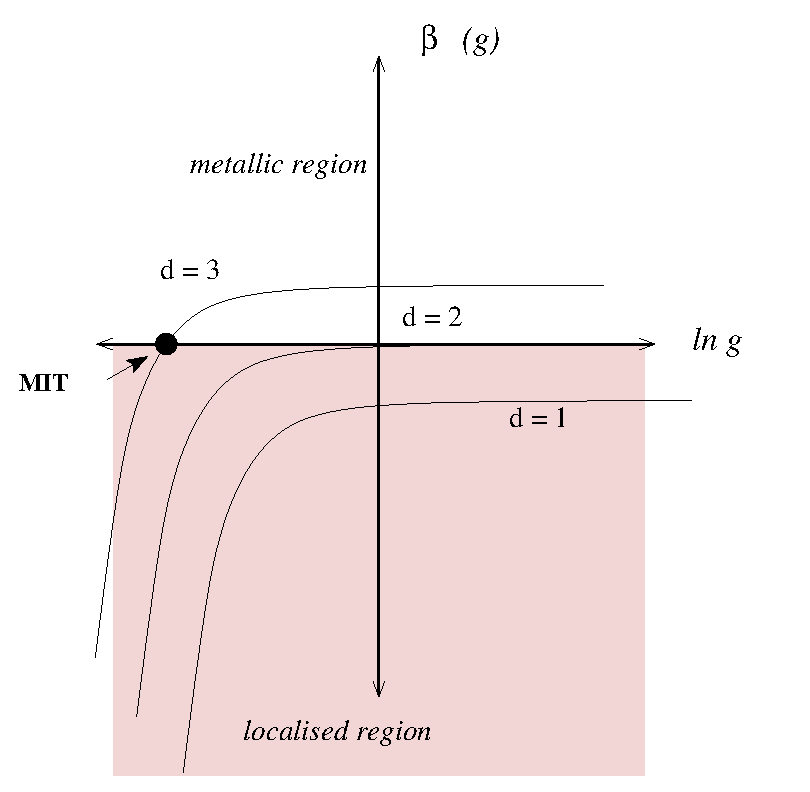
\includegraphics[width=4.0in]{betafxn.eps}
   \caption[ A schematic diagram showing the behaviour of the scaling function $\beta(g)$ for dimensions $d=1,2,3$.]{ A schematic diagram showing the behaviour of the scaling function $\beta(g)$ for dimensions $d=1,2,3$.  The metallic region is $\beta>0$.  The localised region is the shaded part corresponding to $\beta<0$. A crossing point at $\beta=0$ for $d>2$ indicates an MIT.  According to the scale dependence of $\beta(g)$, there are no extended states for $d\leq2$ in the presence of a finite degree of disorder.}
\label{fig-betafxn}
\end{figure}

The scaling theory assumes that $\beta(g)$ is monotonic and that a continuous behaviour connecting the localised and extended regimes is possible.  The scale-dependence of $\beta(g)$ is shown in Fig.~\ref{fig-betafxn}.  When $\beta > 0$ in the metallic case, the conductance increases with $L$ and diverges in the thermodynamic limit.  The asymptotic behaviour of the function is $\beta(g)=d-2$.  For $\beta<0$, $g$ decreases with $L$ and becomes zero as $L\rightarrow\infty$.  In the latter case, $\beta(g)=\ln (g/g_0)$.  The system becomes more metallic or insulating as it gets bigger in $L$.  
For $d\leq2$, $\beta(g)$ is always negative.  This means that in $d\leq2$ unless it is a perfect conductor all electronic wavefunctions will always be localised and the system will always be an insulator in the presence of a finite disorder.
This is not the case for $d=3$.  A crossover at $\beta =0$ between the metallic and insulating regimes exists as seen in Fig.~\ref{fig-betafxn}.  At this critical point, the conductance does not depend on the system size and this scale-invariance implies that exactly at this point there is a metal to insulator transition (MIT).  The set of parameters $x$ such as disorder controls the value of $g(L,x)$.  For instance, if the disorder is weak then the state is in the localised region.  If the disorder is strong enough, it is an extended state.

Near the critical transition, there is only one relevant length scale.  It is the localisation length $\xi$ in the localised regime or the correlation length between wavefunction amplitudes in the extended region.  The localisation (correlation) length diverges near the MIT and since it depends on $x$ then it should diverge at the critical point $x=x_c$ as expressed by \cite{Car87}

%why localisation length diverges
%why is there one relevant length scale

\begin{equation}
 \xi \propto |x-x_c|^{-\nu}.
 \label{eq-XIdef}
\end{equation}
The critical exponent $\nu$ defines the Anderson transition and is the same regardless of the microscopic details for all systems belonging to one universality class or systems sharing the same symmetry in the Hamiltonian.
Furthermore, the scaling theory states that near the critical point of the Anderson transition all systems with finite length $L$ can be scaled by the localisation length for $L\rightarrow \infty$.  If so then the conductance or any measure characterizing critical properties can be described by one scaling function as

\begin{equation}
 g(L,x)=\mathcal{F}\left(\frac{L}{\xi}\right).
 \label{eq-oneparamfxn}
\end{equation}
Equations \eqref{eq-scalelawfxn}, \eqref{eq-scalelawbeta} and \eqref{eq-oneparamfxn} together is also known as one parameter scaling theory \cite{KraM93,MacK81,MacK83}.

%%%%%%%%%%%%%%%%%%%%%%%%%%%%%%%%%%%%%%%%%%%%%%%%%%%%%%%%%%%%%%%%%%%%%%%%%%%%%%%%%%%%%%%%%%%%%%%%%%%%%%%%%%%%%%%%%%%%%%%%%%%%%%%%%%%%%%%%%%%%%%%%%%%%%%%%%%%%%%%%%%%%%%%%%%%%%%%
\section{Numerical Model}
\label{sec-NUMERICS}

To model an electron in a disordered lattice, we use the single-electron tight-binding Anderson Hamiltonian as simply given by
%
\begin{equation}
 \mathcal{H}=\frac{p^2}{2m}+\sum_{i=1}^N U_i(r-R_i),
\end{equation}
%
where $m$ is an effective mass of an electron with momentum $p$, $U_i$ is the potential energy of the $i$-th ion located at $r-R_i$ and the summation is for the total number of ionic sites $N$.
The discrete version of this Hamiltonian in terms of lattice site basis is
%
\begin{equation} \label{anderson_H1} 
\mathcal{H}=\sum_{i} \varepsilon_{i}~\vert i\rangle\langle i\vert + \sum_{i\neq j} t_{ij}~\vert i\rangle\langle j\vert,
\end{equation}
%
for a simple case of only one state per site.
%
Here, $|i\rangle$ is a basis denoting the electronic state localised at position $i=(x,y,z)$ in a cubic lattice of volume $V=L^3$
, $t_{ij}$ are nearest-neighbour hopping amplitudes between sites $i$ and $j$, and $\varepsilon_i$ is the $i$-th site potential energy.  
In this work, we only consider Hamiltonians that fall under the symmetry class of Gaussian orthogonal ensemble, i.e., the $\mathcal{H}$ has time-reversal and spin-rotational symmetries.  The hopping term is set to unity $t=1$ and disorder is introduced into the model by randomising the values of the site potential energies $\varepsilon_i$.
We consider $\varepsilon_i$ to have a uniform probability distribution in the interval $[-W/2,~W/2]$, where $W$ parametrizes the strength of the disorder.  For a critical state at the band centre, $W=W_c\approx16.5$, above the critical disorder $W_c$ all eigenstates are localised \cite{SleMO03,SleMO01,OhtSK99,MilRSU00}.  To minimize boundary effects, periodic boundary conditions are used.
Due to the universality of the Anderson transition, some of the the critical properties such as the critical exponent will not depend on the details of the Hamiltonian.  Hence, a simple tight-binding model for a cubic lattice as just described is able to give the critical properties of the transition.

The $L^3\times L^3$ Hamiltonian matrix has random values in the diagonal elements which represent the site potential energies.  If only nearest neighbor hopping is considered, it is also a sparse matrix with a few off-diagonal elements equal to one.  The matrix is diagonalized using the JADAMILU package \cite{BolN07} which is a Jacobi-Davidson implementation with an integrated solver based on the incomplete-$LU$-factorization package (ILUPACK) \cite{SchBR06, BolN07}.
We have considered eigenstates only in the vicinity of the band centre $E=0$ where the Anderson transition is found when $W_c\approx 16.5$.  We take about five eigenstates in a small energy window around $E=0$ for any given realizations of disorder.

%%%%%%%%%%%%%%%%%%%%%%%%%%%%%%%%%%%%%%%%%%%%%%%%%%%%%%%%%%%%%%%%%%%%%%%%%%%%%%%%%%%%%%%%%%%%%%%%%%%%%%%%%%%%%%%%%%%%%%%%%%%%%%%%%%%%%%%%%%%%%%%%%%%%%%%%%%%%%%%%%%%%%%%%%%%%%%%
\section{Fractal Dimension and Multifractals}
\label{sec-MFABASICS}

%capacity dimension
%Mandelbrot fractal
%characteristic length scale
%Examples of multifractals in nature 

Consider a line segment with unit length $L=1$.  Cover the line with spheres of diameter $l=1/a$.  Other geometrical shapes may be used as well.  The least number of spheres that is needed to fully cover the line segment, $N(l)$, is exactly equal to $(L/l)^{D_f}$ where $D_f$ is called the dimension of the support or simply the dimension of a system.  Extending this to a square and a cube, we can say that $N(l)\propto l^{-D_f}$.  For these three cases of the line segment, square and cube, it is clear to see that $D_f=1,2,3$ respectively.  The value of $D_f$ for the above examples is simply equivalent to the Euclidean or topological dimension.  

Let us now apply the same procedure to a deterministic fractal such as the Mandelbrot-Given fractal as shown in Fig.~\ref{fig-mandelbrot}.  We consider its initial structure which is composed of eight line segments each with length $L=1/3$.  This fractal structure is being generated by replacing each line segment with the initial structure.  For this fractal, $N(l=\frac{1}{3})=8$, that is eight spheres with diameter $l=1/3$ is needed to separately contain each of the eight line segments of the initial structure.  If $l$ is reduced then $N(l=(\frac{1}{3})^2)=8^2$.  Recall that $N(l)\propto l^{-D_f}$, hence $D_f=-\mathrm{\ln}[N(l)]/\mathrm{\ln}[l]$.  For the Mandelbrot-Given fractal, the dimension $D_f$ is a non-integer value of $D_f=\mathrm{\ln}_3 8$ that is less than the Euclidean dimension $d$.  The physical meaning of a non-integer $D_f$ and $D_f<d$ is that the rate at which the volume increases is slower than the increase in linear length $L$.
%
Systems that are defined by one non-integer dimension are called self-similar structures or simply fractals.  Self-similar because they are scale invariant under isotropic scale transformation which means that the volume of the system increases uniformly in every spatial directions. 
Fractals occuring in nature are random fractals.  Their structure could not be exactly formed by repeated generation of a pattern but in a statistical sense they are self similar.
%
\begin{figure}
  \centering
  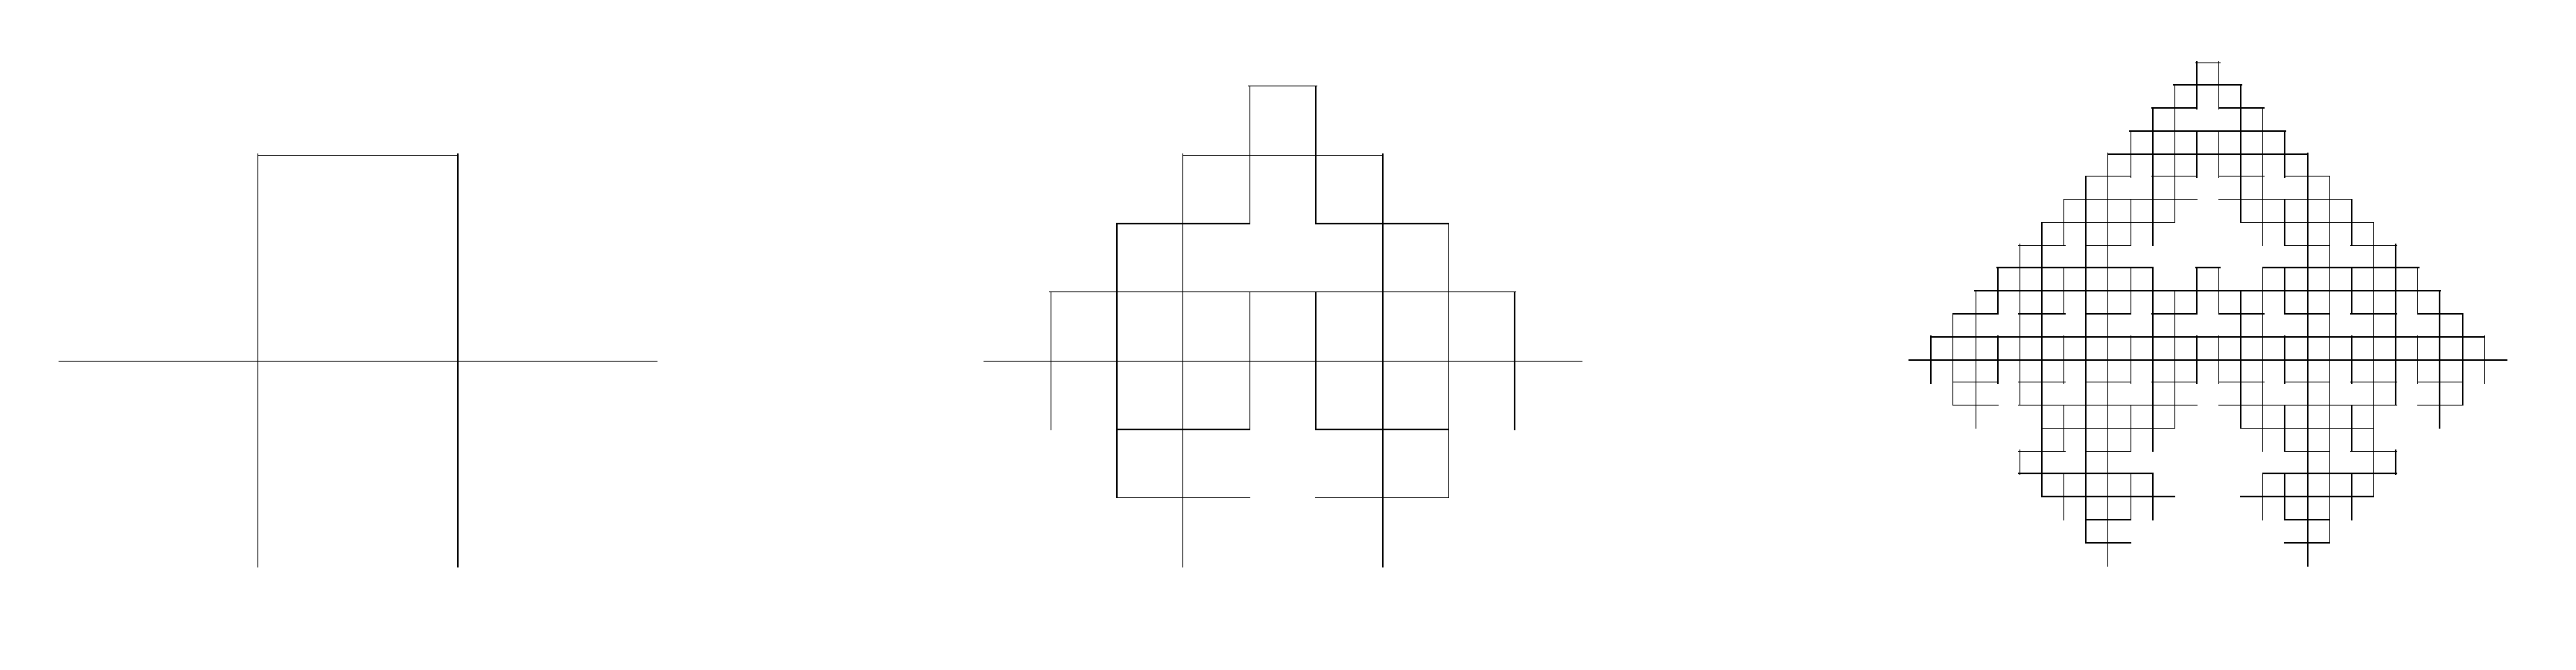
\includegraphics[width=6.0in]{Mandelbrot_Given}
   \caption[The Mandelbrot-Given curve with fractal dimension of $D_f=\ln_3 8$.]{The Mandelbrot-Given curve with fractal dimension of $D_f=\ln_3 8$.  The initial structure shown on the left is composed of eight line segments each with length $L=1/3$.  The higher orders of the fractal structure are generated by replacing each line segment with the initial structure.  Courtesy of K.M. Svensson.
}
\label{fig-mandelbrot}
\end{figure}
%


The dimension that was obtained using the coverage procedure just outlined is called the capacity dimension.  The definition of the dimension in terms of the capacity dimension is useful for the purpose of obtaining the corresponding dimension for a system with random distribution of measures, in particular, for multifractals.
To illustrate the concept of multifractality, we consider the critical eigenstate $|\Psi\rangle=\sum_{i=1}^{L^d}\psi_i|i\rangle$ of an electron at the metal to insulator transition.
Recall that $\vert i\rangle$ is a basis state at site $i$ with wavefunction amplitude $\psi_i$ and the eigenstate is a superposition of all the orthonormal basis states.  This wavefunction corresponds to a three-dimensional cubic lattice of linear length $L$ and volume $V=L^d$.  The wavefunction is normalized such that $\sum_{i=1}^{L^d}\psi_i=1$ and no site has exactly zero $\psi_i$.  This critical state possesses very interesting characteristics.  The values of the wavefunction amplitudes greatly fluctuate from site to site.  Even more, these large fluctuations in $\psi_i$ appear in all length scales, i.e., the fluctuations persist even when the scale at which the eigenstate is observed is varied.  There are points in the wavefunction containing large values of $\psi_i$ and the existence of sites having very small $\psi_i$ such that the distribution function of $\psi_i$ is broad. 
We apply the coverage procedure by dividing the system equally into smaller boxes.  One notices that different boxes enclose different substructures or densities.  The number of boxes enclosing one similar structure gives one fractal dimension.  In fact, a multitude of fractal dimensions is needed to completely characterize the full extent of the complex distribution that defines a system.  Systems of this kind are called multifractals because they are made up of different fractal sets.
This work probes the multifractal characteristics of the electronic eigenstate at the critical point and in the critical regime of the Anderson metal to insulator transition.



















